For our evaluation we decided to mirror the paper's evaluation as closely as possible
to see if we were able to replicate the results obtained there.
Therefore, our baseline is the given implementation of RA in the paper.
Although we compare ourselves to the other implementation, we decided to focus on
replicating the asymptotic results rather than beating the raw performance of their implementation.

\subsection{Experimental Setup}
As already mentioned we want to evaluate similarly to the paper, which means we also mostly varied
window sizes and used sliding granularity of 1 where not specified.
Further information on our data streams can be taken from our Data Generation section \ref{sec:dg}.
To limit the tests and to gain the possibility of rerunning the tests with different configurations
and iterations of our implementation we limited ourselves to 5 million tuples and
a cap of 180 seconds spent only inside our reactive aggregator per run
which sums up to a maximum just short of 6 hours per run of the full evaluation suite.
We ran all tests on a 4-core 2.3 GHz Intel Core i7 with 32 GB of RAM, using
Python 3.7.3 and MacOS 10.15.7.

\subsection{Results and Analysis}
Since we were interested in replicating the papers results, we decided to
recreate figures (in the paper) 6, 8 and 10. Tables 3 and 4 as well as figure 11 were not suitable
for such a comparison while our data sets were not able to guarantee the necessary
(1, 1)-changes for figure 7. Due to the previously mentioned possible bugs in our
implementation we decided to not replicate figure 9. We omitted comparing to figure 12
to keep our focus on the speed of the implementation instead of a memory footprint.

\subsubsection{Comparison for window aggregation from scratch}

\subfile{../figures/figure8.tex}

\begin{figure}[H]
	\centering
	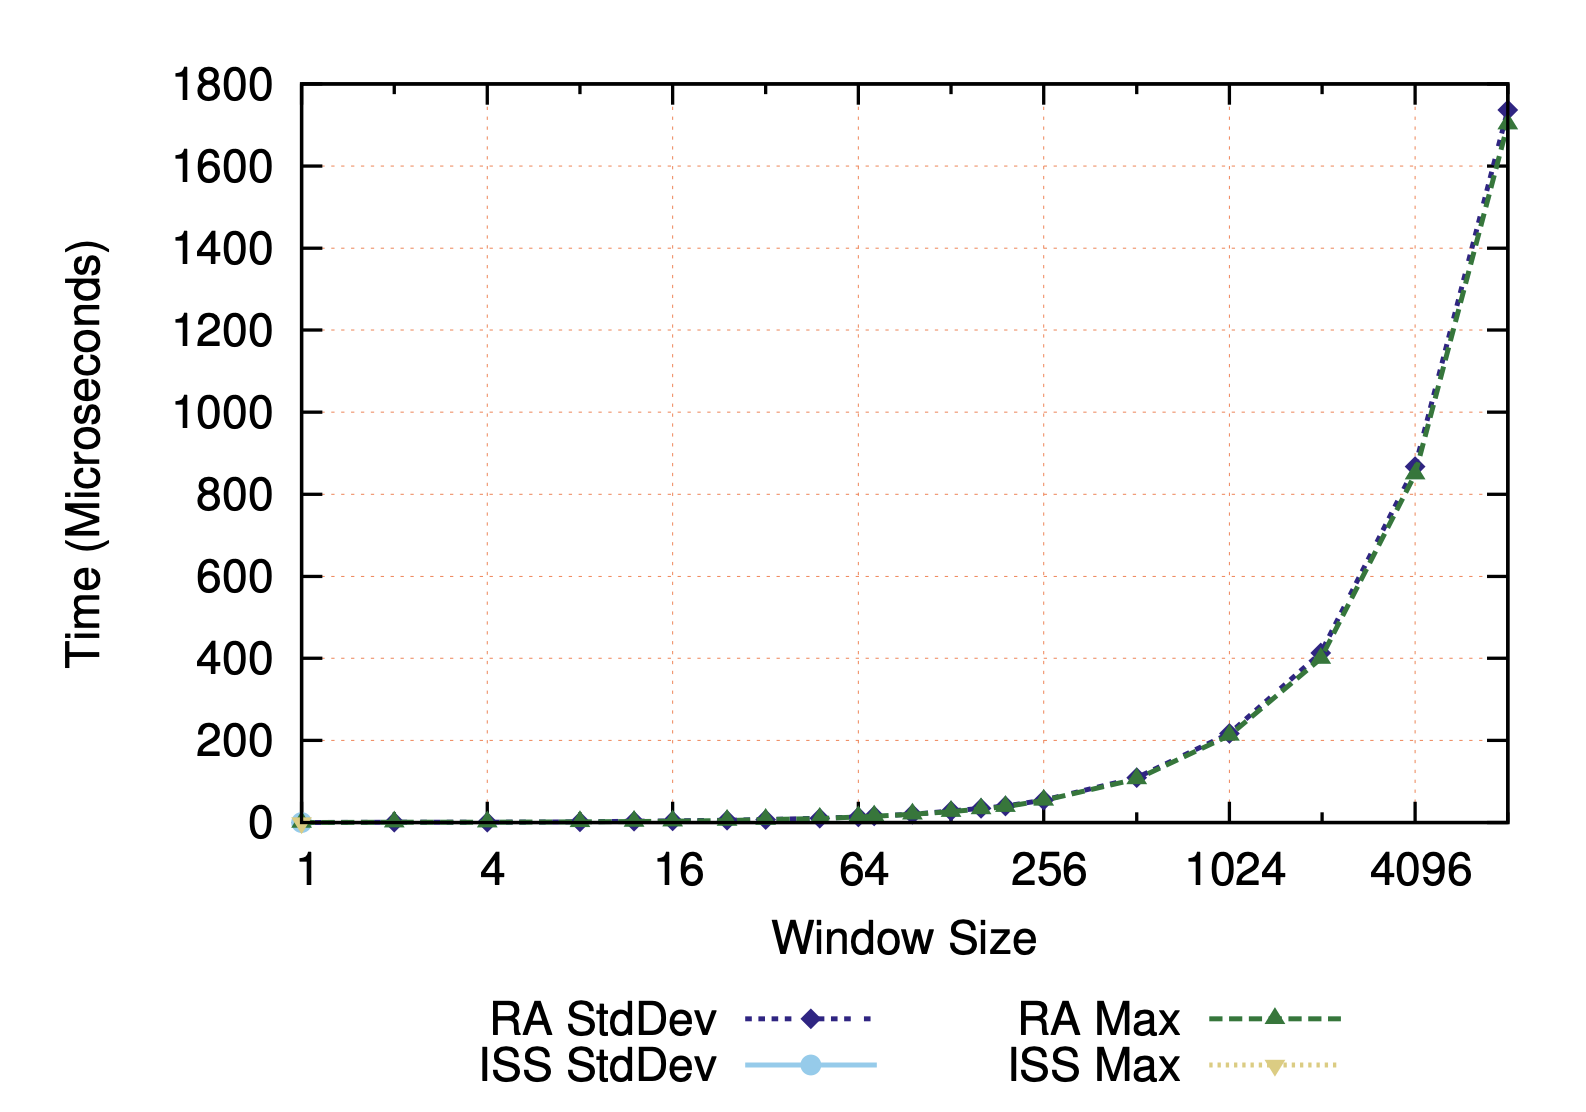
\includegraphics[width=\linewidth]{../figures/fig8}
	\caption{Figure 8 in~\cite{GeneralIncremental15} - Time in microseconds to aggregate the whole window from scratch for different window sizes}
	\label{fig:fig8Orig}
\end{figure}

For replicating figure \ref{fig:fig8Orig} we had almost no expectations. We knew beforehand that
our runtimes would not reach those of the RA from the paper. Nevertheless we decided
to include it as a sort of baseline of our comparison. We were able to reproduce a similar
exponential growth that can be seen in the paper but even roughly comparing the
values shows that our runtimes are much worse. In fact we see that our time is already
more than 50 times worse for window size 1024, even increasing to 245 times for 8192.

\subsubsection{Comparison for throughput}

\subfile{../figures/figure6.tex}

\begin{figure}[H]
	\centering
	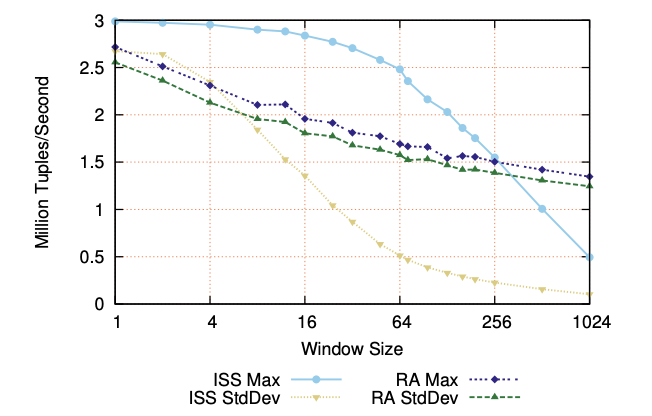
\includegraphics[width=\linewidth]{../figures/fig6}
	\caption{Figure 6 in~\cite{GeneralIncremental15} - Throughput in million tuples per second for different window sizes}
	\label{fig:fig6Orig}
\end{figure}

We hoped to reproduce the asymptotic trend of the throughput in relation to different
window sizes as in the original paper (see figure \ref{fig:fig6Orig}).
Unfortunately, we were not able to reproduce this trend properly (figure \ref{fig:fig6Comp}).
We assume that we may have some problems with our implementation
in a way that omitting front- and back-pointer forced us to search the whole list for
empty spaces. This led to non-constant insertion time as compared to the original
implementation. Nonetheless, we noticed that for window sizes other than powers of
two significant drops in throughput, which we assume to be due to the non-full
binary tree in that case.

\subsubsection{Comparison for average per-tuple cost}

\subfile{../figures/figure10.tex}

\begin{figure}[H]
	\centering
	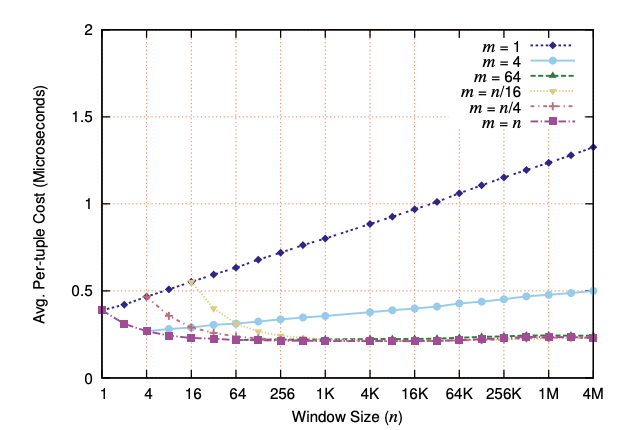
\includegraphics[width=\linewidth]{../figures/fig10}
	\caption{Figure 10 in~\cite{GeneralIncremental15} -  Average tuple cost in microseconds for different sliding granularities and window sizes}
	\label{fig:fig10Orig}
\end{figure}

We hoped to reproduce the asymptotic trend of the average tuple cost in relation
to different sliding granularities (see figure \ref{fig:fig10Orig}), as with figure
\ref{fig:fig6Comp}. Although we stopped our experiments at a way lower window size
due to running times, we already see that the results diverge from the trend of
the original figure as they do not follow the same constant/linear trend.
Nonetheless we see the expected improvements for the different sliding granularities
(figure \ref{fig:fig10CompZoom}) even with our implementation if we focus on the
relevant data range with smaller window sizes.

\subsubsection{Comparison of the evict, insert and update operation runtimes}

\subfile{../figures/ds2-4_comp.tex}

As an extension to the comparisons of the original paper, we decided to include
a test trying to compare the combined insert and evict operations and the update
operation (figure \ref{fig:dsComp}). We expected the datasets with the repeating tuples,
which are exactly the ones using update operations over insert and evict operations,
to be faster because they save one operation. As we see in figure \ref{fig:dsComp}, this
expectation holds true. Additionally, we see that starting with a certain window size,
the runtime stagnates to be constant which we attribute to our datasets, which only
contain 20/500 unique keys, resulting in duplicate events being filtered and the window
not being filled fully.
